
\let\negmedspace\undefined
\let\negthickspace\undefined
\documentclass[a4,12pt,onecolumn]{IEEEtran}
\usepackage{amsmath,amssymb,amsfonts,amsthm}
\usepackage{algorithmic}
\usepackage{graphicx}
\usepackage{textcomp}
\usepackage{xcolor}
\usepackage{txfonts}
\usepackage{listings}
\usepackage{enumitem}
\usepackage{mathtools}
\usepackage{gensymb}
\usepackage[breaklinks=true]{hyperref}
\usepackage{tkz-euclide}
\usepackage{listings}
\usepackage{circuitikz}
\usepackage{gvv}
\begin{document}
\title{Discrete Assignment}
\author{Shravya Kantayapalam\\ EE23BTECH11030}
\maketitle

\begin{enumerate}
    \item \textbf{Question 11.9.4.9}:
    Find the sum to $n$ terms of the series whose $n$th term is given by $n^2 + 2^n$?
 \end{enumerate}  
    \textbf{Solution}:
   

\begin{table}[htbp]
    \centering
    \caption{Input Parameters}
    \begin{tabular}{|l|l|l|}
    \hline
    \textbf{Variable} & \textbf{Description} & \textbf{Value} \\
    \hline
    \( x(n-1) \) & \( n \)-th term of sequence & \( (n^2 + 2^n)u(n) \) \\
    \hline
    \end{tabular}
\end{table}
\begin{align}
x(n-1)&=(n^2+2^n)u(n)\\
2^n \cdot u(n) &\xleftrightarrow{\text{Z}} \frac{1}{1 - 2z^{-1}} \label{eq:11.9.4.9.1}\\
\end{align}
Refer equation\eqref{eq:11.9.5.26.2},equation\eqref{eq:shift} from appendix and equation\eqref{eq:11.9.4.9.1}
\begin{align}
z^{-1}X(z)&=\frac{z^{-1}(z^{-1} + 1)}{(1-z^{-1})^3} +\frac{1}{1 - 2z^{-1}}\\
X(z)&=\frac{z^{-1} + 1}{(1 - z^{-1})^3}+\frac{1}{z^{-1}(1 - 2z^{-1})},\quad{|z|>2}\\
Y(z)&=X(z)U(z)\\
z^{-1}Y(z)&=\brak{\frac{z^{-1}(z^{-1} + 1)}{(1 - z^{-1})^3} +\frac{1}{1 - 2z^{-1}}}\brak{\frac{1}{1-z^{-1}}}\\
z^{-1}Y(z)&=\frac{z^{-1}(1+z^{-1}}{(1-z^{-1})^4}+\frac{2}{1-2z^{-1}}-\frac{2}{1-z^{-1}},\quad{|z|>2}\\
\frac{z^{-1}(1+z^{-1})}{(1-z^{-1})^4}&\xleftrightarrow{Z^{-1}} \frac{n(n+1)(n+2)}{6}u(n)\\
\frac{1}{1-2z^{-1}}&\xleftrightarrow{Z^{-1}} 2^nu(n)\\
y(n-1)&=\frac{n(n+1)(2n+1)}{6}u(n)+2.2^nu(n)-2u(n)\\
y(n)&=\brak{\frac{(n+1)(n+2)(2n+3)}{6}+2^{n+2}-2}u(n)
\end{align}
\begin{figure}[ht]
    \centering
    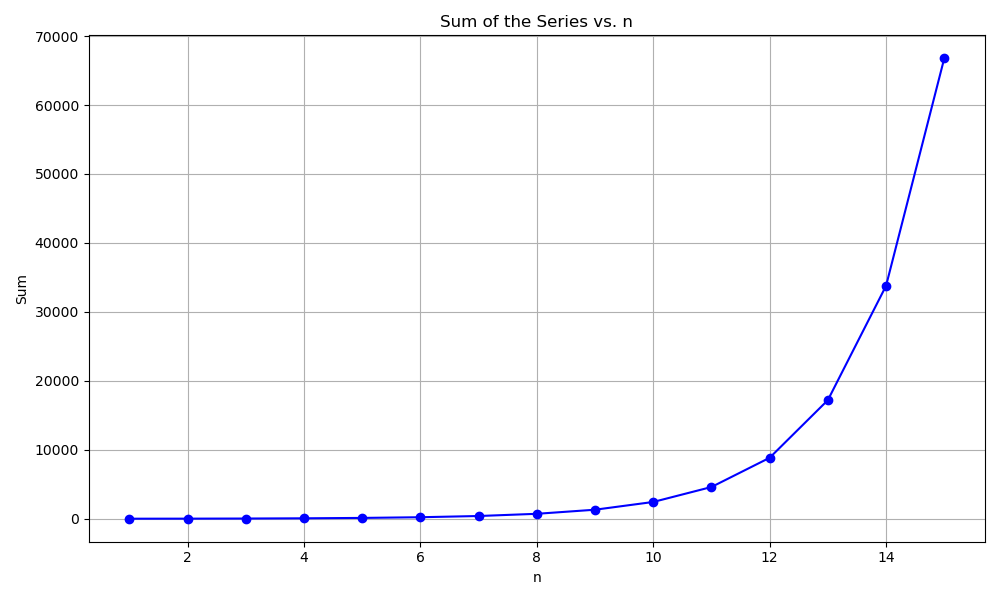
\includegraphics[width=\columnwidth]{figs/main.png}
    \caption{Graph of $y(n)$ for $n \leq 15$ (Graph beyond $n = 29$ is not shown)}
    \label{fig:example}
\end{figure}

\end{document}
